\documentclass[12pt]{article}
\usepackage[utf8]{inputenc}
\usepackage{graphicx}
\graphicspath{{images/}}
\begin{document}
\begin{center}
\huge\underline{``Disruptive Innovation in Healthcare''}
\end{center}
\begin{center}
 
\includegraphics[scale=0.8]{nitlogo.png }
\end{center}
\vspace{1cm}
\begin{center}
   \emph{\large By}\\
\Large{Raj Motwani }\\
\large{Roll No- 21111042}\\
\large{Biomedical 1st Sem}\\
\end{center}
\clearpage
\section{ Consumer devices, wearables, and apps  }

 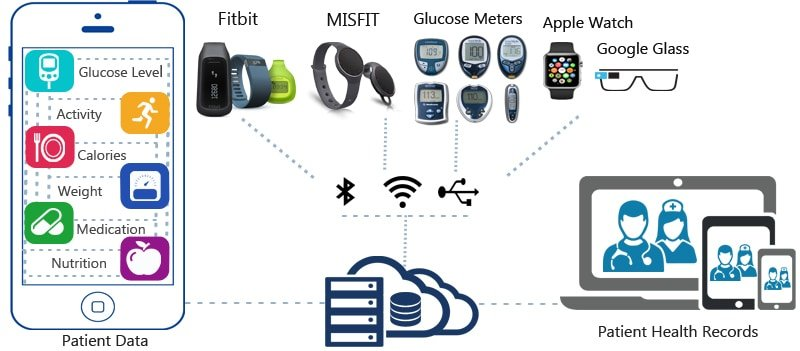
\includegraphics[scale=0.5]{app.jpg }

In the past, a patient could get only biometric data about their pulse, heart rate, blood oxygen, and blood pressure when they went to the doctor’s office. Now, consumers take charge of their own health journey, using data gathered from their Fitbits, smartwatches, and mobile phone fitness apps. Physicians can use the data gathered from these wearables to make treatment decisions, although the vast amount of personal information collected by these apps has led to legal and ethical concerns over data privacy.


\section{AI and machine learning}
 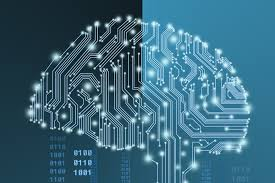
\includegraphics[scale=0.8]{ai.jpeg }


AI applications can manage patient intake and scheduling as well as billing. Chatbots answer patient questions. With natural language processing capabilities, AI can collate and analyze survey responses. AI will probably increase in use as a way to bring down healthcare costs and let doctors and staff focus on patient care. Healthcare leaders must be knowledgeable about the issues surrounding database management and patient privacy. 

\section{Blockchain}
 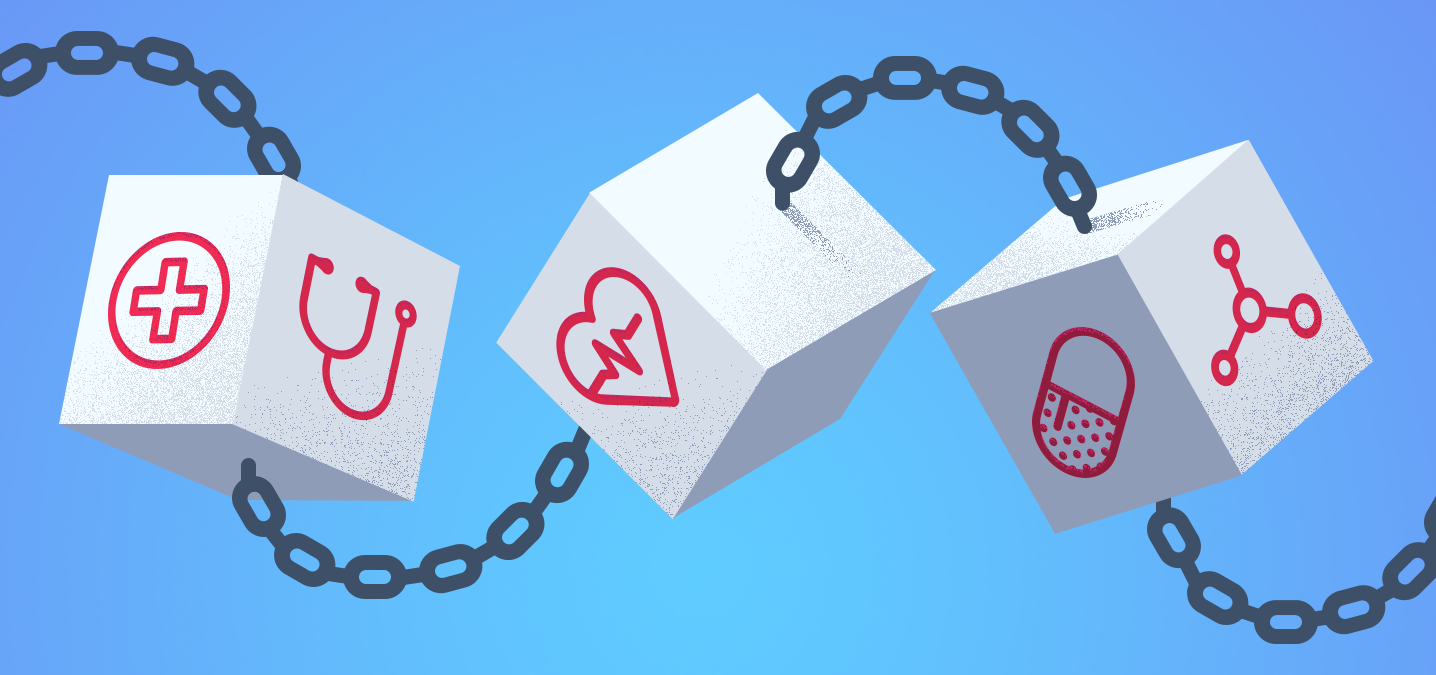
\includegraphics[scale=0.2]{bl.png }

Blockchain is a database technology that uses encryption and other security measures to store data and link it in a way that enhances security and usability. This innovation facilitates many aspects of healthcare, including patient records, supply and distribution, and research. Tech startups have entered the healthcare sector with blockchain applications that have changed how providers use medical data. 

\section{IoT}
 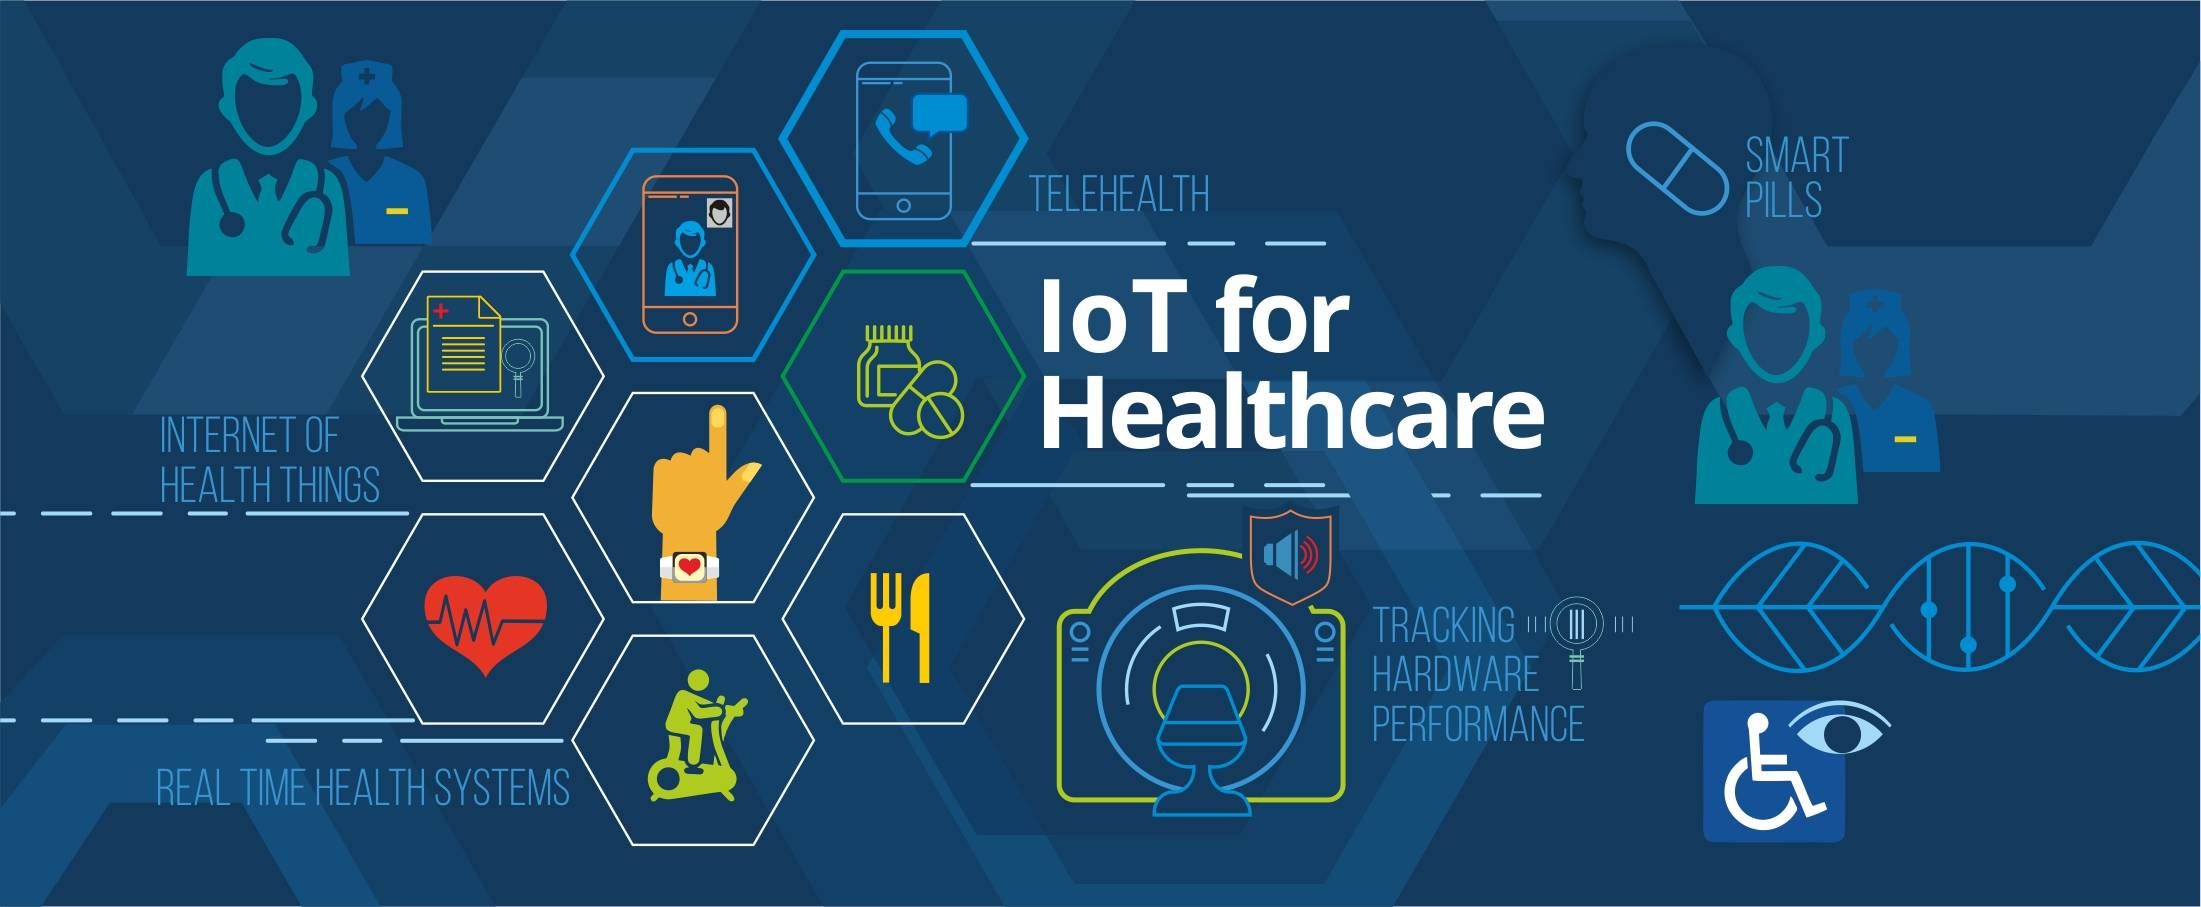
\includegraphics[scale=0.17]{io.jpg }
 \\
What if public health managers could gather data from wearable devices, thermometers, smartwatches, and various other consumer devices — and then use that data to discover disease clusters and provide care to patients more effectively? That’s the vision of the internet of things (IoT). Some of the complex issues surrounding IoT include patient data security and how to define smartwatches — are they consumer products or medical devices that require Food and Drug Administration (FDA) approval?

\section{Electronic health records and big data}

Electronic health records (EHRs) have been a growing part of patient care since the adoption of the Affordable Care Act. The massive amount of EHR data goes far beyond patient health records, however, and can be used to conduct research, improve care, build AI applications, and create new business opportunities. Therefore, healthcare providers have to be aware of the issues surrounding EHR security.

\section{What Are the Key Requirements for Disruptive Innovation?}

To be a successful disruptor, the network of partners—suppliers, contractors, and distributors—must also benefit from the new business model. Certain core requirements include having enabling technology, an innovative business model, and a coherent value network where upstream and downstream business partners benefit from a successful disruption.


\enddocument